\documentclass[12pt,a4paper]{llncs}
\usepackage[utf8]{inputenc}
\usepackage[english]{babel}
\usepackage{lmodern}
\usepackage[T1]{fontenc}
\usepackage[babel=true]{microtype}
\usepackage{amsfonts}
\usepackage{amssymb}
\usepackage{graphicx}
\usepackage{changepage}
\usepackage{hyperref}
\usepackage{xcolor}
\hypersetup{
    colorlinks,
    linkcolor={red!50!black},
    citecolor={blue!50!black},
    urlcolor={blue!80!black}
}
\usepackage{multirow}
\usepackage{footnote}
\makesavenoteenv{tabular}
\makesavenoteenv{table}

\setlength{\fboxsep}{0pt}
\setlength{\fboxrule}{1pt}

\title{Describing Knowledge Organization Systems in BARTOC and JSKOS}
\author{Andreas Ledl\inst{1}  \and Jakob Voß\inst{2}}

\institute{University Library of Basel, Basel
\and Verbundzentrale des GBV (VZG), Göttingen}

\begin{document}
\maketitle
\begin{abstract}
This paper introduces a cooperation between the Basel Register of Thesauri, Ontologies \& Classifications (BARTOC) and project coli-conc to provide information about Knowledge Organization Systems, which ``encompass all types of schemes for organizing information and promoting knowledge management'' \cite{hodge2000systems}, in uniform form. The result is a proper metadata scheme, the JSKOS data format, and an API to connect and access connecting terminology registries so terminologies can be discovered and explored at one place. 
\end{abstract}
\begin{adjustwidth}{2.5em}{2.5em}
\small {\bf Keywords:} knowledge organization systems $\cdot$ terminology registries $\cdot$ metadata schemes
\end{adjustwidth}

\section{Introduction}

Over the last twenty-five years a large amount of Knowledge Organization Systems (KOS)
such as classifications, thesauri, authority files, and term bases have been published online and new ones are added almost daily. Several terminology registries have emerged to identify, describe and make accessible these KOS, ideally in a human- and machine-readable way. These registries replaced link lists, which usually contained information about only a few well-known controlled vocabularies without  elaborated search interfaces or bibliographic description of KOS. The BARTOC terminology registry\footnote{\href{http://bartoc.org/}{http://bartoc.org/}} has quickly evolved to one of the largest collections of information about distinct KOS. This paper summarizes the description of KOS in BARTOC and project coli-conc,\footnote{\href{https://coli-conc.gbv.de/}{https://coli-conc.gbv.de/}} and provision of its metadata as Linked Open Data and the uniform JSKOS data format.

\section{The Basel Register of Thesauri, Ontologies \& Classifications (BARTOC)\protect}

According to Golub et al., who identified four types of KOS registries (Metadata Registries, basic or full Terminology Registries, Service Registries and Data Registries), BARTOC is a basic Terminology Registry, because it contains ``only the metadata of KOS vocabularies'' \cite[1903]{golub2014terminology}. Furthermore, it is a meta registry of KOS registries (see figure~\ref{fig:kos}), linking to 68 other portals.\footnote{\href{http://bartoc.org/en/terminology-registries}{http://bartoc.org/en/terminology-registries}} BARTOC differs from other terminology registries on five counts: it includes \textit{any kind} of KOS from \textit{any subject area} in \textit{any language}, \textit{any publication format}, and \textit{any form of accessibility}. This means that it needs universal systems for formal cataloging, classification and subject indexing of knowledge organization systems.

\subsection{The origins of BARTOC}
The idea for BARTOC has its roots in two classic areas of Library \& Information Science: creating bibliographies and teaching information literacy. On the one hand, it is the latest contemporary descendant of intensive efforts in the 20th century to publish printed surveys of the work on KOS. On the other hand, controlled vocabularies are needed to tag pieces of information and to apply complex search strategies like the ``block building approach'', where a topic is broken down into separate sections to analyze the scope (termino)logically.

It was clear from the start that BARTOC would address the international library community, but also terminologists and scientists from all over the world. Since its launch in November 2013, it has had a total of 300'000 visits and 2.5 million page views.

\subsection{BARTOC's current metadata scheme}
\label{sec:scheme}

BARTOC contains ``a relatively sufficient amount of metadata'' \cite{bratkova2014revue}. The metadata scheme used to describe KOS in BARTOC originates from the early days when BARTOC was just a blog called ``Thesaurusportal''.\footnote{\href{http://www.profi-wissen.de/hilfsmittel-fuer-alle-denkbaren-recherchegebiete-thesaurus-porta/}{http://www.profi-wissen.de/hilfsmittel-fuer-alle-denkbaren-recherchegebiete-thesaurus-porta/}} With migration of the database to Drupal CMS the schema was extended with a mapping to RDF, so KOS description in BARTOC can be used as Linked Open Data. Table~\ref{table:fields} lists all current metadata fields including their mapping to JSKOS (see section~\ref{sec:jskos}) and RDF. The mapping to RDF makes use of schema.org, FOAF, and SKOS ontology.

\begin{table}\centering
\caption{Metadata schema and mappings of KOS description in BARTOC}
\label{table:fields}
\begin{tabular}{lll}
Field & JSKOS & RDF \\
\hline	
URI      & \verb|uri|       & subject URI \\
Title    & \verb|prefLabel| & \verb|skos:preflabel|, \verb|schema:name| \\
Alternative or &
\multirow{2}{*}{\texttt{altLabel}} 
 							& \verb|skos:altLabel|, \verb|schema:name|, \\
English Title               & & \verb|dct:title|, \verb|foaf:name| \\
Author   & \verb|creator|   & \verb|dct:creator|, \verb|schema:creator| \\
Abstract & \verb|scopeNote| & \verb|skos:scopeNote|, \verb|dct:description| \\
Coverage & \verb|subject|   & \verb|dct:subject| \\
Type     & \verb|type|      & \verb|dct:type|, \verb|rdf:type| \\
Format   & -				&  \verb|dct:format| \\
Size     & \verb|extent|    & \verb|dct:extent| \\
License  & -                & \verb|dct:license|, \verb|schema:license| \\ 
Access   & - 				& \verb|dct:rights| \\
DDC      & \verb|subject|   & \verb|dct:subject|, \verb|schema:about| \\
DDC Main Class & -\footnote{\label{fn:s}Only used for searching.} \\
Wikidata & \verb|identifier| & \verb|skos:exactMapping|, \verb|dct:identifier| \\
Link     & \verb|url|       & \verb|schema:url|, \verb|foaf:page| \\
Language & \verb|language|  & \verb|schema:inLanguage|, \verb|dct:language| \\
Topic    & \verb|subject| & \verb|dct:subject|, \verb|schema:about| \\
Year of Creation & \verb|created| & \verb|dct:created| \\
Term Translations  & -\textsuperscript{\ref{fn:s}} \\
VIAF & -\footnote{\label{fn:p}Not refering to the KOS but to its publisher.} \\
Address & -\textsuperscript{\ref{fn:p}} \\
Location & -\textsuperscript{\ref{fn:p}} \\
\end{tabular}
\end{table}

\subsection{Alignment with NKOS AP}

Both BARTOC and JSKOS origin in a bottom-up process by actual description of knowledge organization systems. For this reason the current state is not finished until it has been tested sufficiently in several real-world applications. The Networked Knowledge Organization Systems Dublin Core Application Profile (NKOS AP), created between 2010 and 2015 followed the opposite direction by theoretical investigation of KOS and their registries. The resulting metadata scheme is expected to be ``very important to terminology registries, service registries, vocabulary users (machine or human), and retrieval systems'' \cite{zeng2015nkos}. 
A comparison of the current metadata scheme of BARTOC, JSKOS, and NKOS AP resulted in an overlap at 13 of 28 fields for BARTOC and 18 for JSKOS (table~\ref{tab:nkosap}).

\begin{table}\centering
\caption{Mapping of NKOS AP to BARTOC and JSKOS}
\label{tab:nkosap}
\begin{tabular}{lll}
NKOS AP field & BARTOC & JSKOS \\
\hline	
\verb|dct:title| 		& Title  	& \verb|prefLabel|, \verb|altLabel| \\
\verb|dct:creator| 		& Author 	& \verb|creator| \\
\verb|dct:publisher| 	& Author	& \verb|publisher| \\
\verb|dct:description| 	& Abstract  & \verb|scopeNote| \\
\verb|dct:subject| 		& Coverage, Topic, DDC & \verb|subject| \\
\verb|dct:type| 		& Type 		& \verb|type| \\
\verb|dct:language| 	& Language  & \verb|languages| \\
\verb|dct:identifier| 	& URI, Wikidata & \verb|uri|, \verb|identifier| \\
\verb|dcat:contactPoint| & Link     & \verb|url| \\
\verb|dct:license| 		& License 	& \verb|license| \\
\verb|nkos:sizeNote| 	& Size		& \verb|extent| \\
\verb|dct:format| 		& Format	& - \\
\verb|dct:created|		& Year of Creation & \verb|created| \\
\verb|dct:issued| 		& - 		& \verb|issued| \\
\verb|dct:modified|		& - 		& \verb|modified| \\
\verb|wdrs:describedBy| & -         & \verb|subjectOf| \\
\verb|dct:isPartOf| 		& - 	& \verb|partOf| \\
\verb|prov:wasDerivedFrom| & - 		& \verb|versionOf| \\
\verb|nkos:serviceOffered| & - 		& \verb|concepts|, \verb|types| \\
\verb|dct:audience| & - 			& not defined yet \\
\verb|nkos:basedOn| 	& - 		& not defined yet \\
\verb|nkos:updateFrequency| & - 	& to be discussed \\
\verb|nkos:usedBy| & - 				& to be discussed \\
\verb|nkos:alignedWith| 	& -		& to be discussed \\
\verb|frbrer:isRealizationOf| & - 	& to be discussed \\
\verb|frbrer:isEmbodimentOf| & - 	& to be discussed \\
\verb|dct:relation| 		 & - 	& to be discussed \\
\verb|adms:sample| 			 & - 	& to be discussed \\
\hline
\end{tabular}

%\hspace{0.5em}

%Remaining NKOS AP fields not included in BARTOC and/or JSKOS yet:
%\verb|nkos:sizeNote|, \verb|dct:audience|, \verb|nkos:basedOn|,
%\verb|nkos:updateFrequency|,\\
%\verb|nkos:usedBy|, \verb|nkos:alignedWith|, %\verb|frbrer:isRealizationOf|,
%\verb|frbrer:isEmbodimentOf|, \verb|dct:relation|, and %\verb|adms:sample|.
\end{table}

\subsection{Use of controlled vocabularies to describe KOS}
One particularly special feature of BARTOC, compared to other terminology registries, is its use of controlled vocabularies to describe KOS. It is considered as BARTOC's ``advantage that it specializes in supplementing Dewey’s decimal classification terms (up to the third hierarchic level) \ldots, as well as providing the multilingual EUROVOC thesaurus descriptors'' \cite{bratkova2014revue}. By now the following KOS are referenced. As all KOS also have a record in BARTOC, their corresponding BARTOC URI is also given.

\subsubsection{EuroVoc}
(\href{http://bartoc.org/en/node/15}{http://bartoc.org/en/node/15}) was chosen, although developed especially for the European parliamentary activities, because it is maintained by a trusted authority, it is open data, its domains are multidisciplinary and its terms are available in 25 languages, which is essential for BARTOC's multilingual search. The EuroVoc subject headings are represented hierarchically in the Advanced Search under "Topic". 

\subsubsection{DDC}
(\href{http://bartoc.org/en/node/241}{http://bartoc.org/en/node/241})
is the most widely used library classification system, translated in more than 30 languages. DDC codes up to the third hierarchy level enable grouping different KOS according to a certain field or topic. To make the search interface more easily accessible to wide-ranging groups of users, BARTOC provides DDC numbers and/or captions for content statistics, in the Advanced Search and in faceted search. The service is based on a subscription model. DDC was further expressed as Linked Data \cite{panzer2013dewey} and project coli-conc investigates the connection of DDC to other classification systems so it can be used as mapping backbone with other systems and content.

\subsubsection{KOS Types Vocabulary}
(\href{http://bartoc.org/en/node/1665}{http://bartoc.org/en/node/1665})
was developed by the DCMI NKOS Task Group \cite{KOSTypes} and is, as far as we see, the only controlled vocabulary for KOS types. It differentiates between 14 different types of KOS (categorization scheme, classification scheme, dictionary, gazetteer, glossary, list, name authority list, ontology, semantic network, subject heading scheme, synonym ring, taxonomy, terminology, and thesaurus) and can be found in the Advanced Search under "Type".

\subsubsection{Wikidata}
(\href{http://bartoc.org/en/node/1940}{http://bartoc.org/en/node/1940})
is a general purpose database and authority file that anyone can edit. By now BARTOC only contains mappings to corresponding KOS records in Wikidata to provide links to Wikipedia articles.

\subsubsection{}\hspace{-0.4em}%
Additional vocabularies are used for format, license, and languages of KOS but they have not been published as terminologies yet.
\pagebreak

\begin{figure}\centering
\fbox{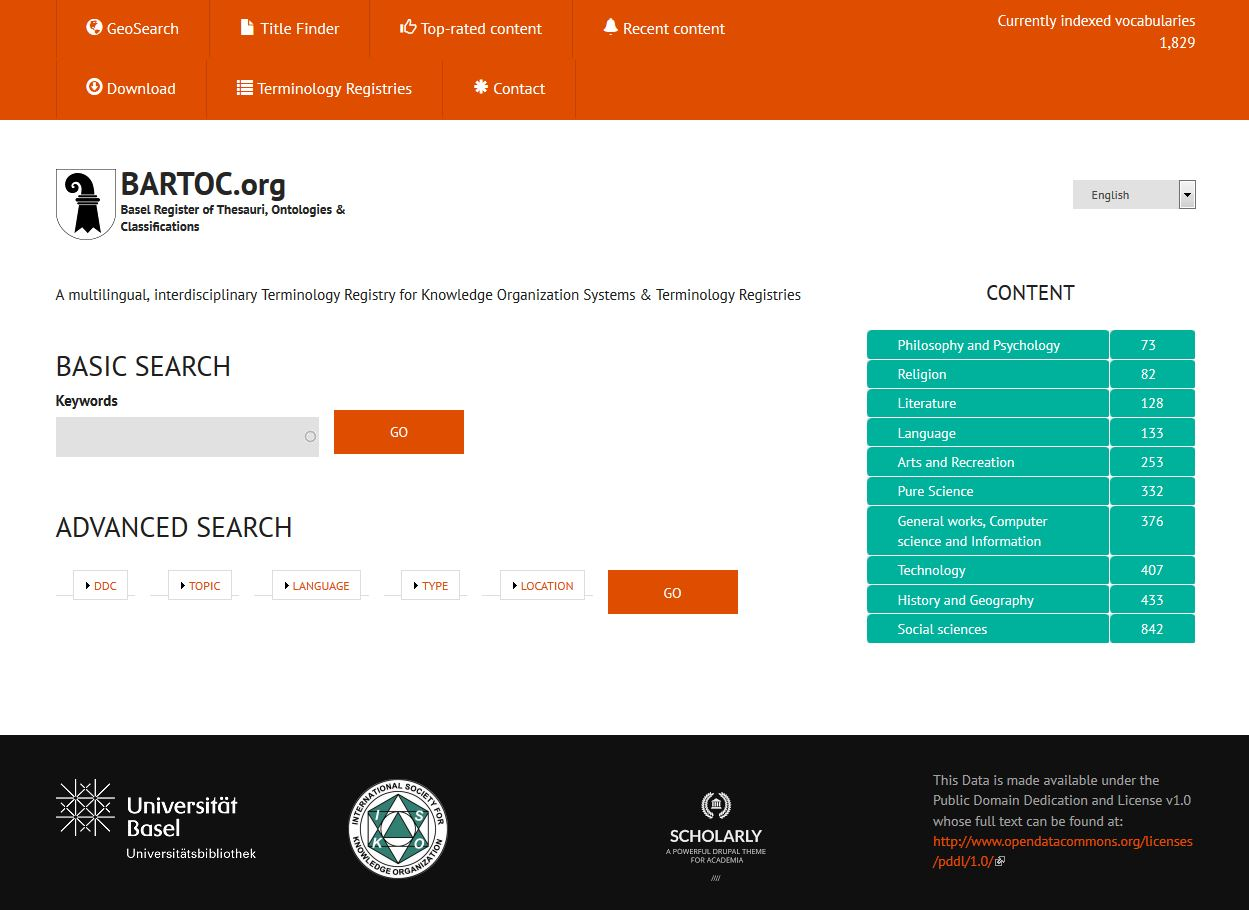
\includegraphics[scale=0.35]{screenshot-bartoc.jpg}}
\caption{Screenshot of BARTOC's search interface}
\end{figure}

\vfill

\section{JSKOS data format for Knowledge Organization Systems}
\label{sec:jskos}
The coli-conc project at Verbundzentrale des GBV (VZG) is funded by German Research Foundation (DFG) to facilitate management and exchange of concordances between knowledge organization systems. This includes the collection and provision of information about KOS and its concepts in a uniform format. To some degree such format is given with the Simple Knowledge Organization System (SKOS) ontology.  SKOS allows the exchange of KOS as Linked Data on the Web but it comes with the complexity of RDF and it requires extensions to cover more than basic properties.
To better support use of KOS data, especially in web applications, the JSKOS data format for Knowledge Organization Systems is precisely defined, tested, and documented \cite{JSKOS}. JSKOS is compatible with JSON-LD\footnote{JSON for Linking Data defines general mapping rules from JSON to RDF.} so it can be converted to SKOS/RDF and vice versa. 

\pagebreak

\subsection{JSKOS metadata scheme}
In a nutshell, JSKOS supports the following object types:

\begin{itemize}

\item \textbf{Concepts} as basic entities of all KOS are covered well by SKOS. JSKOS only adds general fields from Dublin Core and common fields found in authority records.

\item \textbf{Concept Schemes} are equivalent to KOS. In addition to descriptive  fields a link to an API can be provided for querying concepts from this concept scheme.
Figure~\ref{fig:concept-scheme-example} shows EuroVoc as example of a concept scheme  expressed in JSKOS.

\item \textbf{Concept Types} can be used to broadly group concepts, for instance  concepts about places, people, events, and abstract topics.

\item \textbf{Mappings} and \textbf{Concordances} describe mappings between concepts or concept schemes. This is a major contribution of JSKOS because support of mappings in plain SKOS is very limited.

\item \textbf{Registries} collect concepts, concept schemes, concept types, mappings, concordances and/or other registries. Registries have no counterpart in SKOS neither.
\end{itemize}

\noindent
Figure~\ref{fig:kos} illustrates the application of JSKOS objects to BARTOC. The website contains both a terminology registry and a meta registry of other terminology registries. Each KOS in BARTOC can be described as JSKOS Concept Scheme. The concepts of each KOS are not included in BARTOC but project coli-conc provides converters and mappings to make them accessible via downloads and an API. The metadata fields to describe objects in JSKOS are consistent for all object types, for instance \verb|prefLabel| is used for both concept labels and concept scheme titles (see figure~\ref{fig:concept-scheme-example}).

\begin{figure}
\includegraphics[]{kos}
\caption{Overview of metadata about KOS and registries}
\label{fig:kos}
\end{figure}

\begin{figure}
\begin{verbatim}
{
  "@context": "https://gbv.github.io/jskos/context.json",
  "id": "http://bartoc.org/en/node/15",
  "prefLabel": {
      "en": "Multilingual Thesaurus of the European Union"
  },
  "altLabel": { "en": "EuroVoc" },
  "url": "http://eurovoc.europa.eu/",
  "identifier": [ "http://www.wikidata.org/entity/Q1370467" ],
  "type": [
      "http://www.w3.org/2004/02/skos/core#ConceptScheme",
      "http://bartoc.org/en/taxonomy/term/1",
      "http://bartoc.org/en/taxonomy/term/2"
  ],
  "subject": [ {
      "id": "http://dewey.info/class/001",
      "prefLabel": { "en": "Knowledge" }
    }, {
      "id": "http://eurovoc.europa.eu/4060",
      "prefLabel": { "en": "European Union" }
  } ],
  "languages": [ "bg", "ca", "hr", "cs", "da", "nl", "en", "et", "fi",
    "fr", "de", "el", "hu", "it", "lv", "lt", "mk", "mt", "pl", "pt",
    "ro", "sr", "sk", "sl", "es", "sv" ]
}
\end{verbatim}
\caption{Abbreviated JSKOS record of Eurovoc terminology}
\label{fig:concept-scheme-example}
\end{figure}

\subsection{JSKOS-API}
Reusing terminologies does not only require a uniform data format but also methods to access and query selected parts of a KOS. Such methods can be provided either by downloading and importing the whole KOS into a database or by querying an existing service via API. Several APIs and services exist for selected KOS (for instance WebDewey\footnote{\url{http://dewey.org/webdewey/}. This service is based on a subscription model.} for DDC) but without common standard and many terminology provider avoid the technical effort of setting up and maintain an additional web service. For this reason project coli-conc defines JSKOS-API based JSKOS and evaluation of similar APIs.

The JSKOS-API Specification\footnote{See \href{https://gbv.github.io/jskos-api/}{https://gbv.github.io/jskos-api/} for the current draft.} is still in an early state of development. Nevertheless KOS services have been implemented to access DDC, Wikidata, and the Integrated Authority File (GND). 
Based on JSKOS-API applications can make use of any KOS that is available in JSKOS format. Figure~\ref{fig:normdatenservice} shows a general terminology service (``Normdatendienst'') of VZG that provides search and browsing interface to multiple terminologies.
The implementation is published as open source and can be used in other sites as well.\footnote{All software created in project coli-conc is published at GitHub. A current list of software can be found at \href{https://coli-conc.gbv.de/publications/}{https://coli-conc.gbv.de/publications/}.}


\begin{figure}
\centering
\fbox{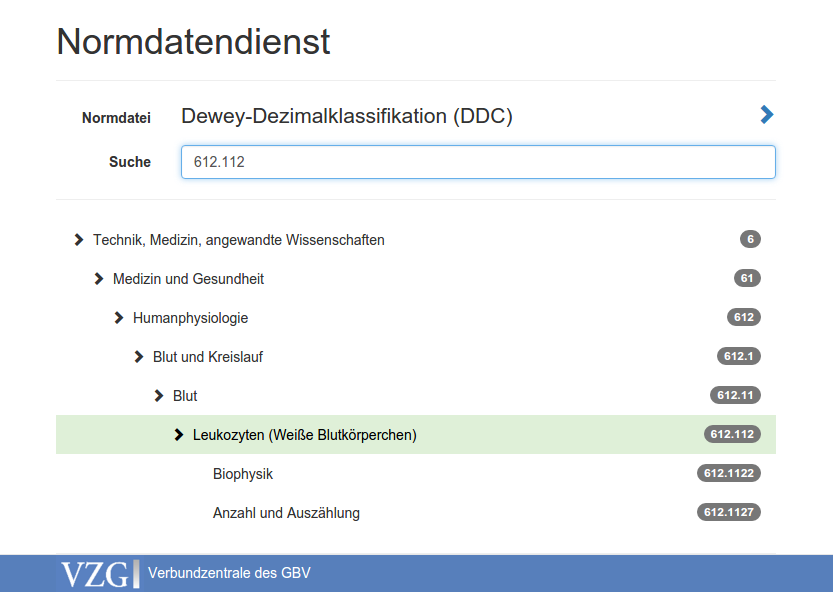
\includegraphics[scale=0.38]{screenshot-normdatenservice-ddc.png}}
\caption{Screenshot of VZG Terminology Service}
\label{fig:normdatenservice}
\end{figure}

% To facilitate use of terminologies it not only requires a un

\section{Summary}

The Basel Register of Thesauri, Ontologies \& Classifications prepares thousands of Knowledge Organization Systems under one interface in order to achieve greater visibility, to highlight their features, to make them searchable and comparable, and to foster knowledge sharing.\footnote{See \cite[20]{hlava2011developing}}
BARTOC covers a lot of user tasks, allowing ``to find, identify, select, obtain \ldots KOS resources through the data provided'' \cite[1906]{golub2014terminology}. When a user has found an interesting terminology, he or she is directed to the publisher's site for further investigation. But once the KOS is made available via JSKOS-API, its concepts and structure can directly be explored from other places as well. 
The publication of more and more KOS via JSKOS-API, as being implement in project coli-conc, will allow users to directly browse and search in KOS from BARTOC. In reverse, the content of BARTOC registry will be searchable from other sites as well. 

Due to the mutual benefit for both, BARTOC and coli-conc, it will be the most urgent task to improve alignment of BARTOC metadata scheme, NKOS AP metadata scheme, and JSKOS data format.
The advantages of the latter, compared to plain RDF, include ease of use, a uniform description also for mappings, concordances, and registries, and a defined method to query registries and concept schemes. This way both BARTOC and JSKOS(-API) will foster the visibility, availability and usefulness of Knowledge Organization Systems in general.

\bibliographystyle{splncs03}
\bibliography{bibliography.bib}
\end{document}
